\documentclass[8pt,twocolumn,letterpaper]{article}


\setlength{\textheight}{10.5in}
\setlength{\textwidth}{7.225in}
\setlength{\columnsep}{0.28in}
\setlength{\topmargin}{-0.8in}
\setlength{\leftmargin}{-0.8in}
\setlength{\headheight}{-0.2in}
\setlength{\headsep}{0in}
\setlength{\parindent}{1pc}
\setlength{\oddsidemargin}{-.304in}
\setlength{\evensidemargin}{-.304in}


\usepackage{times}
\usepackage{epsfig}
\usepackage{graphicx}
\usepackage{amsmath}
\usepackage{amssymb}
\usepackage{comment}
\usepackage{epsfig}
\usepackage{listings}

\usepackage[left=1cm, right=1cm, top=1cm, bottom=1.1cm]{geometry}
\usepackage{titlesec}
\titlespacing*{\section}
{0pt}{0.75ex}{0.75ex}
\titlespacing*{\subsection}
{0pt}{1.5ex}{0.75ex}

\usepackage{amsmath}
\DeclareMathOperator*{\argmax}{argmax} % thin space, limits underneath in displays
\usepackage[colorlinks=true, citecolor=green, linkcolor=blue, urlcolor=blue]{hyperref}


\usepackage{graphicx, caption, subcaption}



\setcounter{page}{1}
\begin{document}

%%%%%%%%% TITLE
\title{Report for Mini-Project 2 "Probabilistic Parser for French"}


\author{Yonatan \bsc{DELORO}\\
{\tt\small yonatan.deloro@eleves.enpc.fr}
% For a paper whose authors are all at the same institution,
% omit the following lines up until the closing ``}'f'.
% Additional authors and addresses can be added with ``\and'',
% just like the second author.
% To save space, use either the email address or home page, not both
}


\maketitle
%\thispagestyle{empty}

\small
%%%%%%%%% ABSTRACT
The goal of this project was to build a statistical constituency parsing architecture, using the CYK algorithm and handling out-of-vocabulary words (OOV). In this short report, I first describe the architecture of the system, then I discuss the results. \\

\textit{\textbf{Statement} : I wrote personally the whole code of the system, except the functions given in the Polyglott embeddings tutorial [1] I imported. The system I developed does not rely on any function from a parsing library (such as NLTK). However, I made use of the NETWORKX library, to have a tree structure in order to move easily from the parsing in Chomsky form to a non-binary parsing. Besides, the graphical representations of the trees in the report's annex were plotted using PYGRAPHVIZ but the import is not necessary to use the system (cf. README). Finally, I made use of PYEVALB library for scoring purposes only.}\\

\section{The developed system}

\subsection{Extraction of the PCFG Grammar}

First module, "pcfg", enables to extract a probabilistic context-free grammar from the training corpus. More precisely, it decomposes into : (i) a "grammar", which stores the probability of each rule $X_0 \rightarrow X_1....X_n$ encountered : 
$P(X_0 \rightarrow X_1....X_n) = \frac{C(X_0 \rightarrow X_1....X_n)}{\sum_{Y} C(X_0 \rightarrow Y)}$ (where $Y$ denotes any possible right-hand term), (ii) and a "lexicon", which stores for each part-of-speech (POS) tag $X$, the frequencies of the words annotated with such tag, ie. $P(X \rightarrow w) = \frac{C(X \rightarrow w)}{\sum_{w'} C(X \rightarrow w')}$  (I found it more convenient to have the probabilities sum to 1 for a given POS - instead of a given token - as these will be the probabilities used by the CYK parser [2]).  In addition to these two components, the "pcfg" module also keeps tracks of the frequencies of the words and of the tags in the training corpus.

Finally, I added a function enabling to binarize the grammar, as the CYK algorithm, in its canonical form, can handle only rules with two non pre-terminal symbols at the right hand.
Therefore, I applied the two rules BIN and UNIT of the Chomsky Normalization process [3]. I implemented the BIN rule, exchanging each rule $X_0 \rightarrow X_1....X_n$  ($n>2$ non-terminal symbols) with the following $n-1$ rules : $X_0 \rightarrow X_1Y_1$, $Y_1 \rightarrow X_2Y_2$, ...,  $Y_{n-2} \rightarrow X_{n-1}X_n$, introducing new artificial tags (if not done before), and transferring the counts of the original rule to the ones of the new rules. Besides, I implemented the UNIT rule to get rid of rules $X \rightarrow Y$ : if $Y$ was a POS tag, I introduced $X\&Y$ a new symbol such that  $X\&Y \rightarrow w$ for any $Y \rightarrow w$ (same counts but multiplied by $P(X \rightarrow Y)$) and $U \rightarrow VX\&Y$ for any $U \rightarrow VX$; otherwise I created $X \rightarrow Y_1Y_2$ for any $Y \rightarrow Y_1Y_2$ (same counts but multiplied by $P(X \rightarrow Y)$). (Of course, I binarized the grammar before converting counts into probabilities.)

\subsection{Handling OOV}

The second module I developed, called "oov", enables to assign the closest token of the lexicon to any unseen token, and returns "None" if it judges no word is enough similar to be assigned similar POS tags. Closeness is based defined on edit distance and word embedding similarity. More precisely, given an OOV word : 

\textbf{1) Normalization} I first try various normalizations (numbers replaced by "\#", case) to see if one of these new tokens actually matches a word of the lexicon. 

\textbf{2) Embedding similarity} If (1) fails, I try various normalizations of the word to see if one belongs to the words having an embedding in the Polyglot database. If so, I return the word of the lexicon $L$ whose embedding, if it exists, is the closest to the embedding of the queried OOV $q$. "Closest" is understood as the one which maximizes the cosine similarity between the two embeddings, or equivalently, since I normalized the embeddings, the one which minimizes their Euclidian distance : $min_{l \in L} ||\phi(q)-\phi(l)||^2 = ||\phi(q)||^2 + ||\phi(l)||^2 - 2\phi(q)^T\phi(l) = 2(1-cos(\phi(q),\phi(w)))$. Embeddings of lexicon words are precomputed for faster parsing.

\textbf{3) Spelling correction} If (2) fails, I try to correct the spelling of the word. To do so, I chose to compute the Levenhstein distance in Damerau version (to also allow for swaps) with each word of the lexicon, and I return the most frequent candidate in the training corpus among the ones achieving the minimal distance. However, if the minimal distance is greater than 4, I return "None" (max. number of mistyping errors per word is generally of this order). Previously, I was also computing the distance with each word having a Polyglot Embedding and if such a word not in the lexicon decreased the minimal distance, I was looking for its closest lexicon word in terms of embeddings. However, this took too much time in practice so that I just let it as an option (cf. code). I computed the distance using dynamic programming. Denoting $d(i,j)$ the distance between sequence $s$ until character $i$ and sequence $s'$ until $j$, we get (i) if $i,j > 1$, $s[i-1]=s'[j]$ and $s[i]=s'[j-1]$ : $ d(i,j) =\min \{d(i,j-1)+1,d(i-1,j)+1,
&d(i-1,j-1) + 1_{s[i]=s[j]}, d(i-2,j-2) + 1\}$ , (ii) otherwise $ d(i,j) =\min \{d(i,j-1)+1,d(i-1,j)+1,
&d(i-1,j-1) + 1_{s[i]=s[j]}\}$ (first term corresponds to inserting $s'[j]$, second to removing $s[i]$, third to substituting $s[i]$ by $s'[j]$ (paying nothing if these are the same !), and fourth to swapping $s[i-1]$ and $s[i]$ (if there is a swap)).
    
An OOV word is assigned the probability of the tags of the closest token found, and if no closest token is found, is assigned the frequencies of the POS tags in the training corpus.



\subsection{Parsing with CYK algorithm}

Given that I removed grammar rules with unique or more than two non-terminal symbols at the right hand, I can apply a probabilistic version of the CYK algorithm to parse the sentence. Let's denote $P(s,l,X)$ the probability of the most likely tree parsing the sub-sentence of length $l+1 \in [1,n]$, starting at word position $s \in [0,n-l-1]$, and tagged $X$, of the sentence to parse ($n$ words). If $l\geq 1$, we can compute : \begin{align*}P(s,l,X) = \max_{0 \leq c \leq l-1, ~ X \rightarrow YZ} & P(X \rightarrow YZ) \times P(s,c,Y) \\ & \times P(s+c+1,l-c-1,Z)\end{align*} ($Y$ tags subsentence from $s$ to $s+c$ and $Z$ subsentence from $s+c+1$ to $s+l$). And we have $P(s,0,X)= C(X \rightarrow word(s))$. Therefore, I used dynamic programming (looping with increasing $l$) to compute $P(0,n-1,SENT)$. If $P(0,n-1,SENT)=0$, then no valid parsing was found. Otherwise, in order to find the parsing reaching such probability, I also stored on the fly the decomposition $<c,Y,Z>$ enabling to reach $P(s,l,X)$ at any update. In order to speed up, I also precomputed a new storing of the grammar $g$ with nested dictionnaries and where $g[i][j][k]$ stores $P(S(i)\rightarrow S(j)S(k))$ (where $S$ denotes the tag stored with index $k$). Therefore, if $P(s,c,Y)$ was lower than the current $P(s,l,X)$, cut $c$ is not optimal and I could avoid to look at any decomposition $X \rightarrow YZ$ for such cut. This saved time since the many artificial symbols introduced with the Chomsky BIN rule were systematically the second symbol of a rule's right hand term. Though, the parsing remains quite slow for large sentences. 

Thanks to the CYK algorithm, we end with the most likely parsing tree, which is however binary and contains artificial symbols introduced by BIN/UNIT rules. What I do to retrieve parsings in the same shape as the ones of the SEQUOIA corpus is to link the children of any symbol introduced by BIN with its own father, and to split any symbol $X\&Y$ introduced by UNIT into two nodes : $X\&Y$ becoming $X$ and having a child $Y$ whose own child is the token (former child of $X\&Y$).

\section{Results}

The parsing system was built using the first 80\% of SEQUOIA as training corpus. I did not make use of the next 10\% (but I provide some potential use of a validation set in section 3). And I tested the parser on the last 10\% ie. the last 310 last sentences.

The resulting grammar contains 40 part-of-speech tags and 4316 artificial symbols introduced  by Chomsky normalization (4293 introduced with BIN and 23 with UNIT). Lexicon contains 8958 words, of which 7427 (original/normalized form) possess a Polyglot embedding. In total, there are 100.004 embeddings in the Polyglot database.

Out of the 310 test sentences, my parser found 283 valid parsings. Tagging accuracy (proportion of correct POS tags assigned to words) was 92.3\% (excluding the non-parsed sentences) and 86.2\% (counting an accuracy of 0 for each word of a non parsed sentence).  Among the non-parsed sentences, we can notably find specific structures : book references, quotings, splited composite nouns (eg. \textit{"hommes politiques -cles"}), subject-verb inversion (eg. \textit{"restent encore aux mains de divers groupes terroristes les passagers d'un bateau de plaisance"}). 

In Figure 1, we can see that the tagging accuracy does not decrease with the length of the sentence, but the number of mistakes, the bracketing precision and bracketing recall do, which is not unexpected.  

Finally, the OOV module does not make weird choices (Figure 2), but often it happens that the OOV word does not have a Polyglot embedding and is at a spelling distance more than 4 to any lexicon word : in such cases I preferred not to assign a closest word but to rely on general tags frequencies, which maybe harms a bit the performances. 


\begin{figure}[h!]
    \centering
      \begin{subfigure}[b]{0.8\linewidth}
        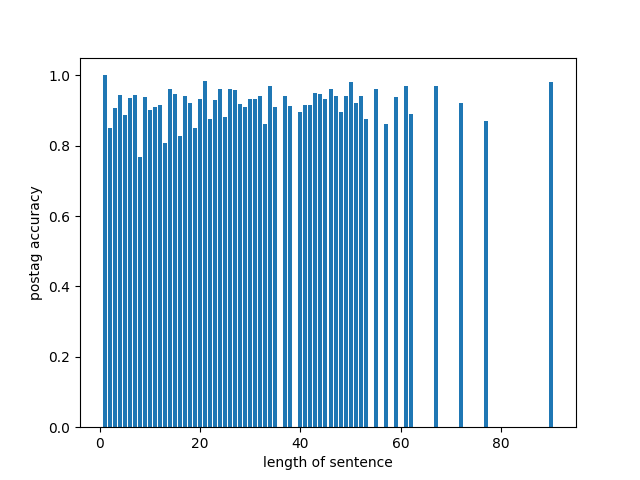
\includegraphics[width=\linewidth]{report/1.png}
    \end{subfigure}
    \begin{subfigure}[b]{0.8\linewidth}
        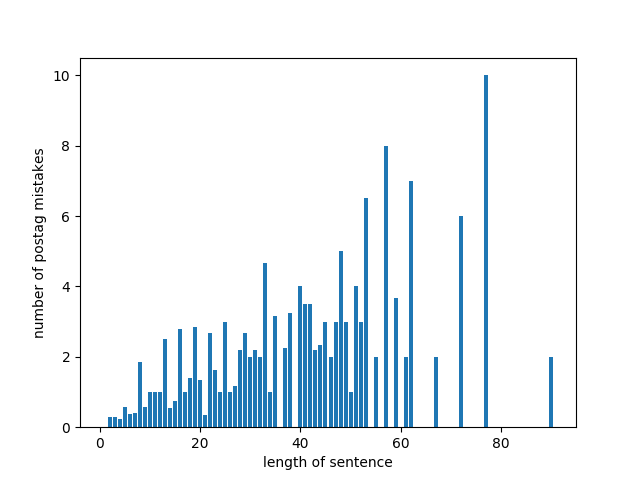
\includegraphics[width=\linewidth]{report/2.png}
    \end{subfigure}
     \begin{subfigure}[b]{0.8\linewidth}
        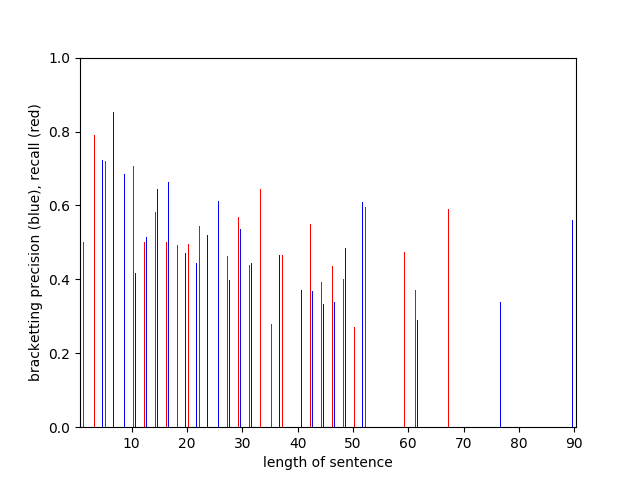
\includegraphics[width=\linewidth]{report/3.png}
    \end{subfigure}
    \caption{Tagging accuracy (proportion of correct POS tags), number of mistakes (incorrect POS tags), bracketing precision and recall, against sentence length on the 283/310 parsed sentences of SEQUOIA test set.}
    \label{mrcnn}
\end{figure}

\begin{figure}[h!]
\begin{center}
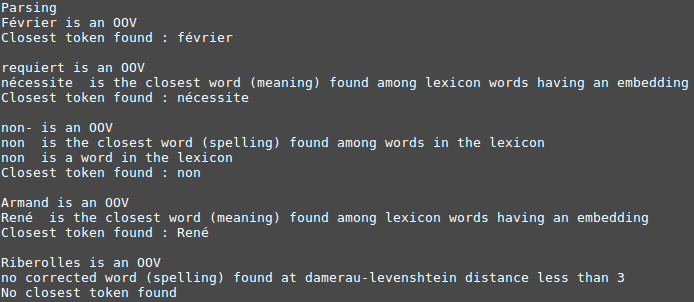
\includegraphics[scale=0.4]{report/spelling.png}
\caption{Examples of decisions taken by the OOV module on OOV words of test sentence 2.}
\end{center}
\end{figure}

\section{Paths for improvements}

Below are the three paths I would have followed to improve the parser with more time :

1) First of all, the spelling corrector could definitely be sped up, building for instance a Levenshtein finite state transducer, which would have probably allowed to introduce the words with Polyglot embeddings as candidates. 

2) In addition, instead of looking for the most frequent correction candidate among the ones at minimal distance, I could have use tables of probabilities for misspellings (ex : substitution of character $x$ by $y$) as well as a bigram language model, in order to compute the probability of a correction $c$ for word $w$ following word $v$ in the sentence as $P_{Bigram}(c|v) \times \prod_{o \in O(w \rightarrow c)} P_{correction}(o)$ where $O(w \rightarrow c)$ is the set of operations enabling to reach the minimum edit distance. If so, I would have for instance used the validation set to calibrate the smoothing parameters of the bigram language model. 

3) I would have also worked on optimizing even more the data structures used for the implementation of the CYK algorithm, since the parser is not very fast currently.

\begin{thebibliography}{5}  

[1] Tutorial on Polyglot Embeddings : https://nbviewer.jupyter.org/gist/aboSamoor/6046170 \\

[2] Daniel Jurafsky & James H. Martin, Speech and Language Processing, 2018 \\

[3] Wikipedia pages : "CYK algorithm" and "Chomsky normal form"

\end{thebibliography}

\onecolumn


\section*{ANNEX :} Example of a relatively good parsing. Sentence 89 of the test corpus (24 words). \\ Accuracy (proportion of correct postags) : 0.92, bracket precision : 0.86, bracket recall : 0.80, done in 11.61s.


\begin{figure}[h!]
\begin{center}
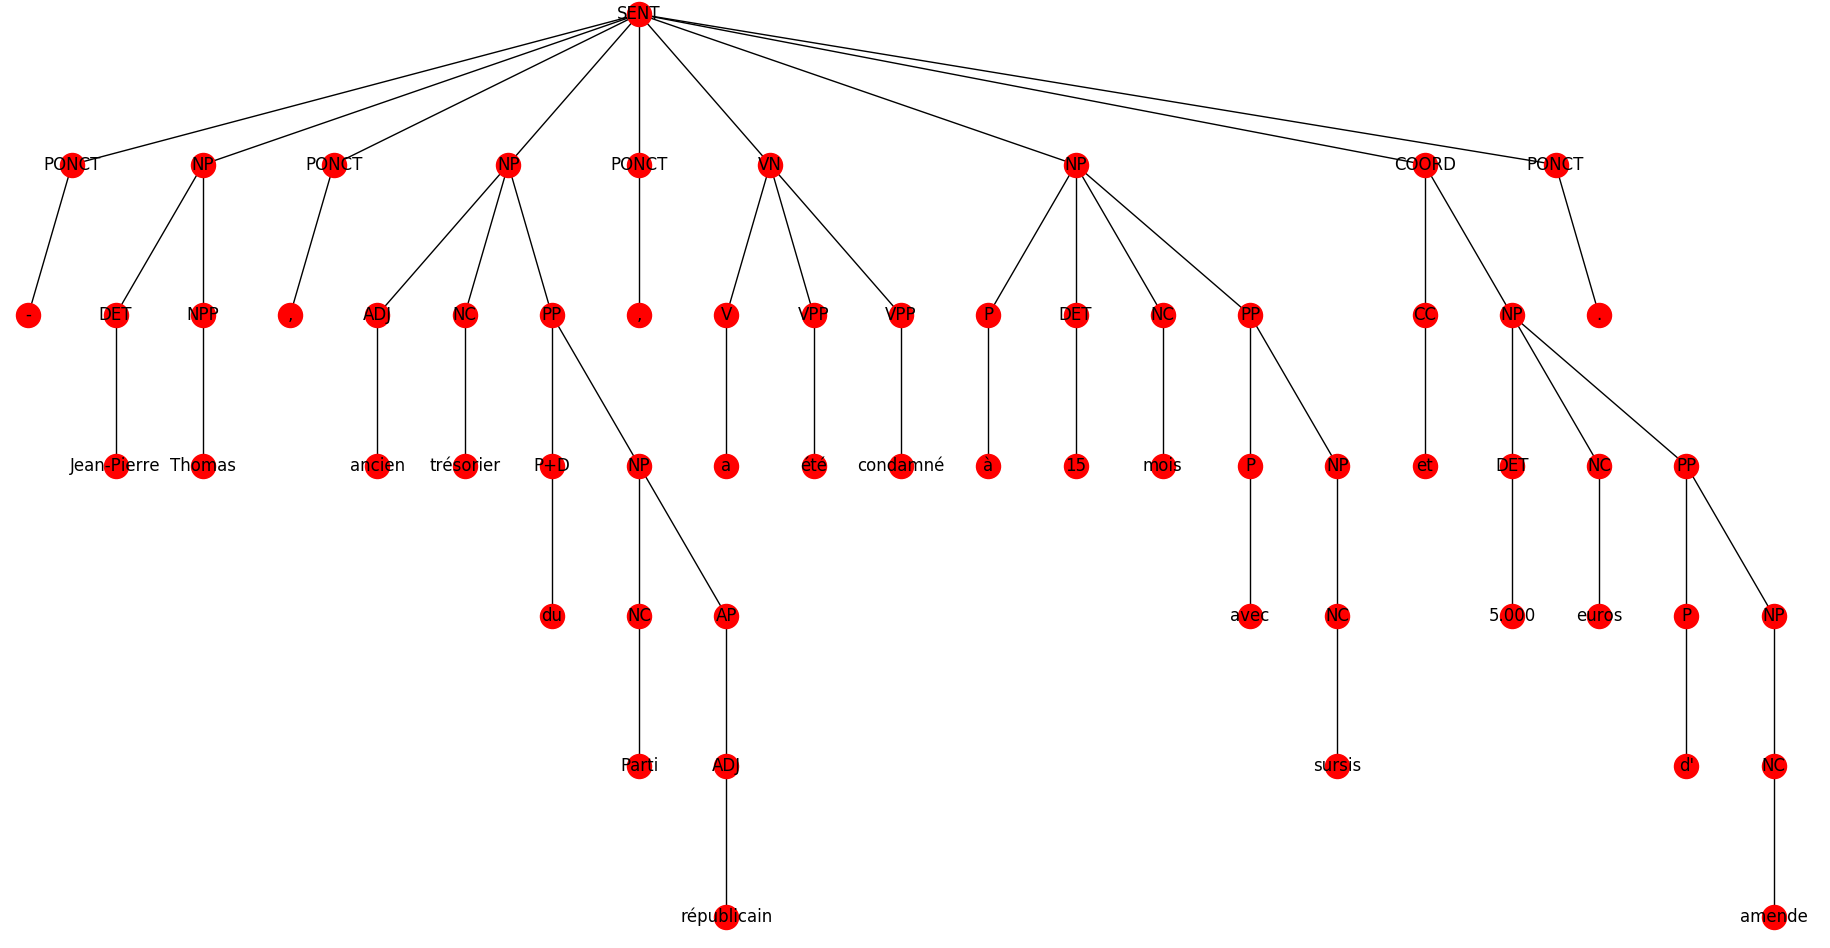
\includegraphics[scale=0.3]{report/my_parsing.png}
\caption{My parsing (after removal of artificial symbols introduced with Chomsky normalization).}
\end{center}
\end{figure}


\begin{figure}[h!]
\begin{center}
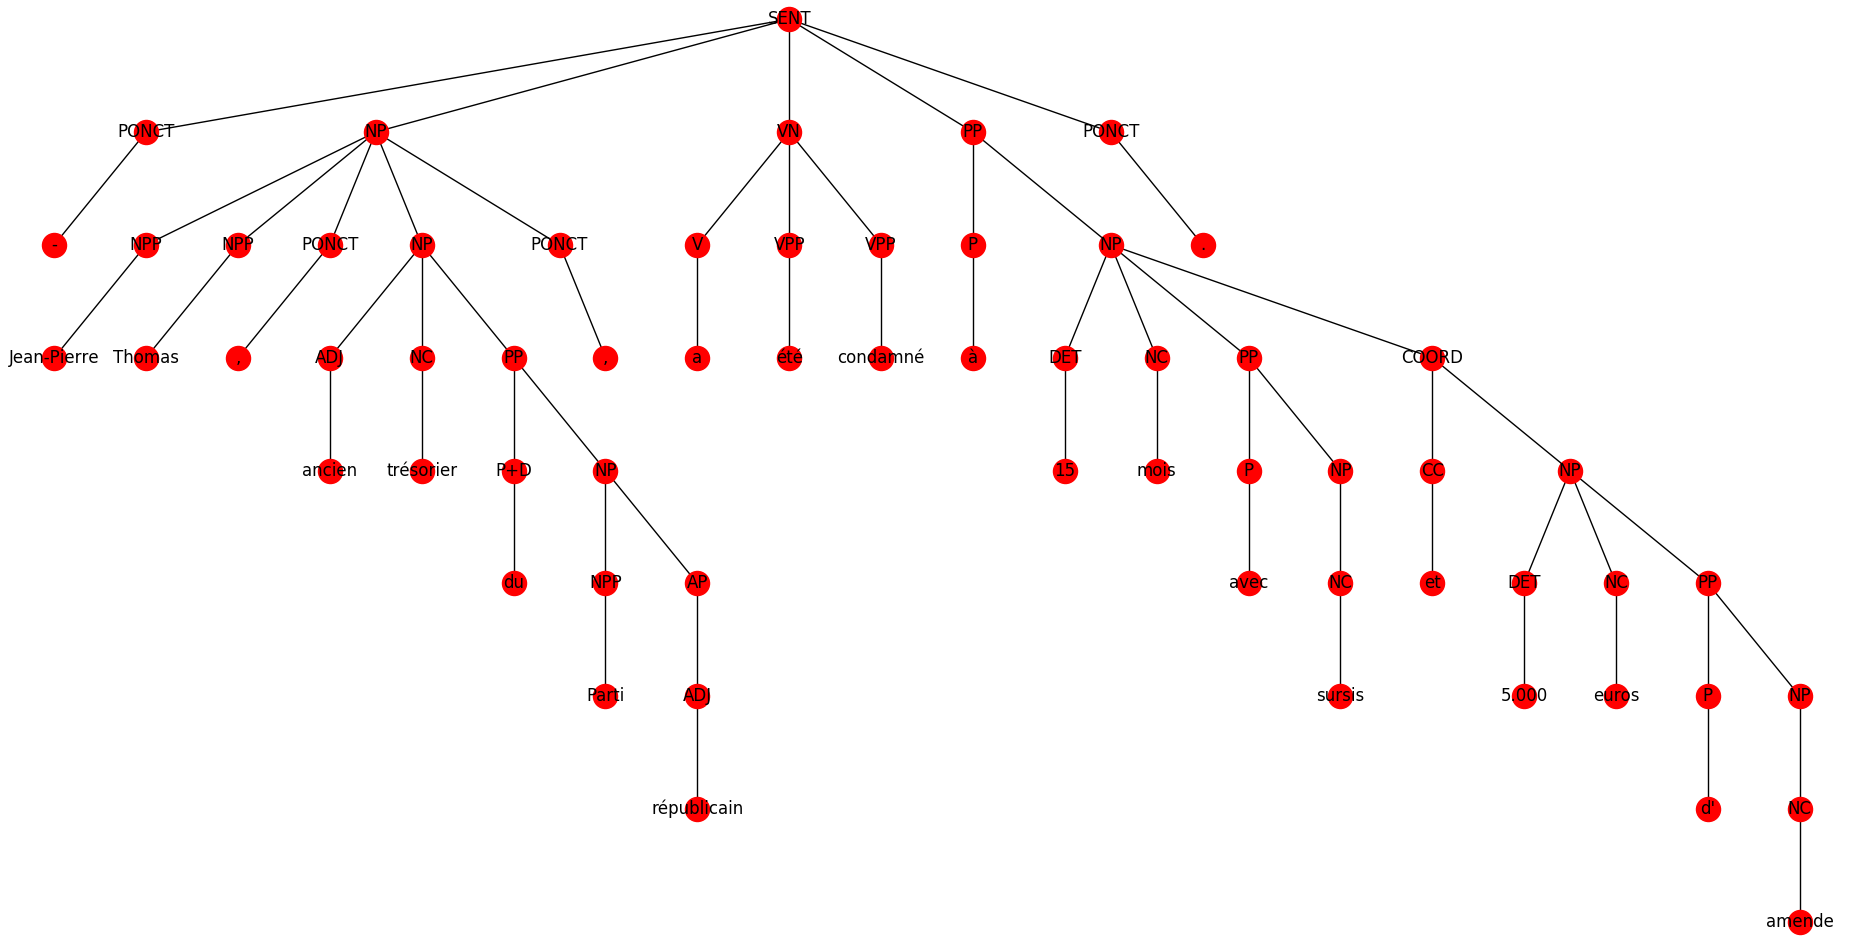
\includegraphics[scale=0.3]{human_parsing.png}
\caption{Gold parsing (SEQUOIA).}
\end{center}
\end{figure}

\end{document}

    



